\documentclass[11pt,a4paper]{article}
\usepackage[utf8]{inputenc}
\usepackage[margin=2.5cm]{geometry}
\usepackage{amsmath}
\usepackage{booktabs}
\usepackage{graphicx}
\usepackage{float}
\usepackage{caption}
\usepackage{enumitem}
\usepackage{xurl}
\usepackage[hidelinks]{hyperref}
\graphicspath{{../results/figures/}}
\captionsetup{font=small,labelfont=bf}
\setlist{itemsep=2pt,topsep=4pt}

\title{\textbf{As is, where is: does a tabular foundation model need the table cleaned first?}\\[6pt]
\large TabPFN-3.5 against 2013-style feature engineering on the Kaggle \emph{Blue Book for Bulldozers} auction data}
\author{Agnaldo Calvi Benvenho\thanks{BP Avalia\c{c}\~oes e Per\'icias Ltda., S\~ao Paulo, Brazil. Mechanical engineer, machinery and equipment appraiser and court-appointed expert. Code and results: \url{https://github.com/abenvenho/tabpfn-bluebook-bulldozers} (Apache-2.0).}}
\date{October 2026}

\begin{document}
\maketitle

\begin{abstract}
\noindent Used machinery is auctioned \emph{as is, where is}: in the condition it stands, without warranty or cleanup. We ask whether a tabular foundation model can price under the same clause, taking the data as published. TabPFN-3.5 receives the 2013 Kaggle \emph{Blue Book for Bulldozers} auction table exactly as released, with the manufacturing year recorded as 1000 for 9.5\% of the sales, the hour meter missing for 64\% and zero for another 18\%, 35 of 51 predictor columns more than half empty and the sale date as text. It is used zero-shot through the Prior Labs API and compared with a LightGBM given 2013-style cleaning and feature engineering. Every model is given sales through 2011 only (all 401,125 of them for the primary run and the baseline) and predicts the 11,573 sales of January--April 2012. Five hypotheses and their refutation rules were committed before the first run. The raw table scores RMSLE 0.2200 against 0.2325 for the engineered baseline (paired bootstrap difference $-0.01245$, 95\% CI $[-0.01480, -0.01021]$), and its 80\% predictive interval covers 82.0\% of the realized prices. Cleaning or joining the ``corrected'' Machine Appendix improves TabPFN-3.5 by less than the pre-registered margin. One hypothesis is refuted: the most recent sales beat a random sample of equal size only for small contexts, and lose at 200,000 sales. On the same evaluation sales, the only published model we found, a tuned random forest, scores 0.2396.
\end{abstract}

\noindent\textbf{Keywords:} tabular foundation models; TabPFN; machinery and equipment valuation; auction prices; data cleaning; pre-registration; out-of-time evaluation.

\section{Introduction}

Valuing used heavy equipment from auction records is routine work for appraisers, lenders and insurers, and the records are dirty. Manufacturing years are missing or entered as placeholders, hour meters are blank or reset, configuration fields are filled for some sales and not others, and the same machine model appears under thousands of codes and free-text descriptions. In practice, a large share of the modelling effort goes into cleaning and engineering this table before any model is fitted.

Tabular foundation models change where that effort may be needed. TabPFN \cite{hollmann2023,hollmann2025} is pre-trained on synthetic tables and predicts a new table in context: the training rows are passed together with the rows to predict, and no model is fitted to the data at hand. If such a model can price from the table as published, the cleaning step stops being a prerequisite.

We test that claim on a canonical dirty benchmark, the 2013 Kaggle \emph{Blue Book for Bulldozers} competition \cite{kaggle2013}, under a design set against it. The bet is that TabPFN-3.5, with no cleaning and no tuning, prices the following months' sales as well as a gradient-boosting model \cite{friedman2001,ke2017} given 2013-style cleaning and feature engineering. Following a falsificationist reading \cite{popper1959}, the bet is split into five hypotheses, each with a numeric rule that would refute it, committed to version control before the first TabPFN run.

The contributions are: (i) a pre-registered, out-of-time comparison of a zero-shot tabular foundation model with an engineered gradient-boosting baseline on raw auction data; (ii) a decomposition of the effect of cleaning, external corrected attributes, context size and context sampling; (iii) a reproducible pipeline whose API spend is quoted by the server and read from the usage counter after each block; and (iv) the findings, including one refutation.

\section{Related work}

The 2013 competition asked for the auction price of heavy equipment from usage, type and configuration. Published write-ups by top-ranked teams share a recipe: separate models per product group or subgroup, hyper-parameter search, the removal of old or atypical periods and, in two of the three, blends of gradient boosting machines, random forests \cite{breiman2001} and linear models \cite{seroussi2014,olariu2013,dataiku2013}. The same teams report that the ``corrected'' Machine Appendix released by the organisers did not help or made results worse; one of them used it only to fill missing values. Parr and Howard \cite{parr} use the competition's validation set as a test set for a tuned random forest, which provides the only published reference we found on the basis used here.

TabPFN was introduced as a transformer that solves small classification problems in a forward pass \cite{hollmann2023} and extended to regression \cite{hollmann2025}; later versions, including TabPFN-3.5, are served through the Prior Labs API \cite{priorlabs}. Its claims are usually tested on curated benchmarks; this study asks what happens on a table that was never curated, against a baseline that was.

\section{Data}

\subsection{Source and splits}

The competition files contain 53 columns: the sale identifier, the price and 51 predictors. The split is by time, as published by the organisers (Table~\ref{tab:splits}). The validation prices were released by Kaggle after the competition (\texttt{ValidSolution.csv}); the test prices never were. The raw files are not redistributed with the code; they are available at the competition page after accepting its rules.

\begin{table}[H]
\centering\small
\caption{Data splits, as published by the competition.}
\label{tab:splits}
\begin{tabular}{lllr}
\toprule
Set & Period & Role here & Sales \\
\midrule
Train & 1989-01-17 to 2011-12-30 & context / training & 401,125 \\
Valid & 2012-01-01 to 2012-04-28 & evaluation, prices from \texttt{ValidSolution.csv} & 11,573 \\
Test & 2012-05-01 to 2012-11-16 & submission file only; prices withheld & 12,457 \\
\bottomrule
\end{tabular}
\end{table}

\subsection{What is dirty}

Table~\ref{tab:dirt} groups the 51 predictors and reports what was measured on the training sales. In total, 35 of the 51 columns are more than half empty. Prices range from US\$4,750 to US\$142,000, with a median of US\$24,000. A separate Machine Appendix holds ``corrected'' attributes for 358,593 machines: manufacturing year, manufacturer and size class.

\begin{table}[H]
\centering\small
\caption{Predictor groups and measured defects in the 401,125 training sales.}
\label{tab:dirt}
\begin{tabular}{p{4.0cm}rp{9.0cm}}
\toprule
Group & Cols. & Defects \\
\midrule
Machine and model identity & 7 & 5,218 model codes; series empty in 86\%, descriptor in 82\% \\
Class and size & 4 & 74 product classes described in text; size empty in 53\% \\
Age and use & 3 & year = 1000 in 9.5\%; hour meter empty in 64\% and zero in 18\%; usage band empty in 83\% \\
The sale & 4 & date as text (\texttt{3/14/2012 0:00}); 53 state values; auctioneer empty in 5\% \\
Configuration options & 33 & 30 of 33 more than half empty; 26 also use the text ``None or Unspecified'' \\
\bottomrule
\end{tabular}
\end{table}

\section{Methods}

\subsection{Target and metric}

All models predict $\log(1+\text{price})$ and are scored with the competition's metric,
\begin{equation}
\mathrm{RMSLE} = \sqrt{\frac{1}{n}\sum_{i=1}^{n}\bigl(\log(1+\hat{y}_i) - \log(1+y_i)\bigr)^2},
\end{equation}
which measures relative error. Predictions and quantiles are back-transformed with $\exp(\cdot)-1$.

\subsection{TabPFN-3.5}

TabPFN-3.5 is called through the Prior Labs API (\texttt{tabpfn-client} 0.6.1) with default settings, zero-shot: no fitting to these data, no hyper-parameter search. Each run returns the mean prediction and the quantiles 0.10, 0.25, 0.50, 0.75 and 0.90; the 80\% interval is [q10, q90]. Three versions of the table (\emph{arms}) are compared:
\begin{itemize}
\item \textbf{raw} (primary): the 51 predictors as parsed from the CSV, including the sale date as text; nothing imputed or corrected (before upload, \texttt{tabpfn-client} itself removes commas and repeated spaces from text values, in every arm);
\item \textbf{clean}: 2013-style cleaning; years before 1900 and zero hour readings set to missing; the date replaced by year, month, day of week and days since 1989; age at sale added;
\item \textbf{appendix}: the raw table plus six Machine Appendix attributes joined on the machine identifier.
\end{itemize}
The primary context is all 401,125 training sales. It was chosen by a rule committed in advance (the largest of all sales, 200k, 100k or 50k that fits the daily quota), applied to the server's cost quote of 181,897 tokens per call before any result was seen. For the context hypothesis, contexts of 200k, 100k and 50k sales are drawn as the most recent sales or as a random sample (seed 42). Two further modes are explored outside the hypotheses: \emph{fast} (the \texttt{v3.5-fast} model) and \emph{thinking} (extra fit-time search, here optimising RMSE on the log scale; capped by the API at 200k rows, point predictions only).

\subsection{Baselines}

The \textbf{median} baseline predicts the training median (US\$24,000) for every sale. The \textbf{LightGBM} baseline \cite{ke2017} receives the clean arm's cleaning and features (55 features), with text columns as native categorical features. Hyper-parameters are fixed: learning rate 0.05, at most 128 leaves, at least 20 sales per leaf, 80\% of columns and rows sampled per tree, seed 42. The number of trees is chosen by early stopping (patience 200, at most 5,000) on the most recent 10\% of training sales (40,084 sales after 2010-10-30), with no 2012 data; the model is then refitted on all training sales with the selected 995 trees. Unlike the 2013 top teams, it uses no per-group models, no blending and no hyper-parameter search.

\subsection{Protocol and hypotheses}

Hypotheses, thresholds and analysis rules were committed to git before the first TabPFN run on the real data (Table~\ref{tab:hyp}). Paired comparisons use a bootstrap over the 11,573 validation sales \cite{efron1993}: 10,000 resamples with replacement, seed 42, percentile 95\% interval of the RMSLE difference. A materiality margin of 0.005 RMSLE applies to H1 and H2. A script applies the rules and writes the verdicts; an independent AI agent, which had not taken part in producing the results, recomputed every number in the repository's README with its own code.

\begin{table}[H]
\centering\small
\caption{Pre-registered hypotheses and refutation rules.}
\label{tab:hyp}
\begin{tabular}{lp{7.2cm}p{5.6cm}}
\toprule
 & Hypothesis & Refuted if \\
\midrule
H1 & Raw TabPFN-3.5 is not worse than the engineered LightGBM & worse by $>0.005$ RMSLE with 95\% CI above 0 \\
H2 & Cleaning, or joining the Machine Appendix, does not improve TabPFN-3.5 & improvement $>0.005$ with CI above 0 \\
H3 & At equal context size, the most recent sales beat a random sample & RMSLE(recent) $-$ RMSLE(random) $\geq 0$ at any size \\
H4 & The 80\% interval holds four months ahead & coverage outside 75--85\% \\
H5 & The primary run scores in the 2013 top 10\% on the leaderboard-mirror split & RMSLE $>0.25339$ \\
\bottomrule
\end{tabular}
\end{table}

\section{Results}

\subsection{Verdicts}

Table~\ref{tab:verdicts} gives the pre-registered verdicts and Figure~\ref{fig:runs} every configuration. Four hypotheses survive; H3 is refuted.

\begin{table}[H]
\centering\small
\caption{Pre-registered verdicts on the January--April 2012 sales. Differences are RMSLE of the first model minus the second; negative means the first errs less.}
\label{tab:verdicts}
\begin{tabular}{lllll}
\toprule
 & Difference & Value & 95\% CI & Verdict \\
\midrule
H1 & raw $-$ LightGBM & $-0.01245$ & $[-0.01480, -0.01021]$ & corroborated \\
H2 & raw $-$ clean & $+0.00175$ & $[+0.00083, +0.00270]$ & corroborated (below margin) \\
H2 & raw $-$ appendix & $+0.00267$ & $[+0.00150, +0.00388]$ & corroborated (below margin) \\
H3 & recent $-$ random, 50k & $-0.00639$ & $[-0.00839, -0.00440]$ & supports \\
H3 & recent $-$ random, 100k & $-0.00032$ & $[-0.00215, +0.00152]$ & supports by the rule; tie \\
H3 & recent $-$ random, 200k & $+0.00234$ & $[+0.00079, +0.00389]$ & \textbf{refutes} \\
H4 & 80\% interval coverage & 82.0\% & band 75--85\% & corroborated \\
H5 & primary RMSLE & 0.22001 & threshold 0.25339 & corroborated, with caveat \\
\bottomrule
\end{tabular}
\end{table}

\begin{figure}[H]
\centering
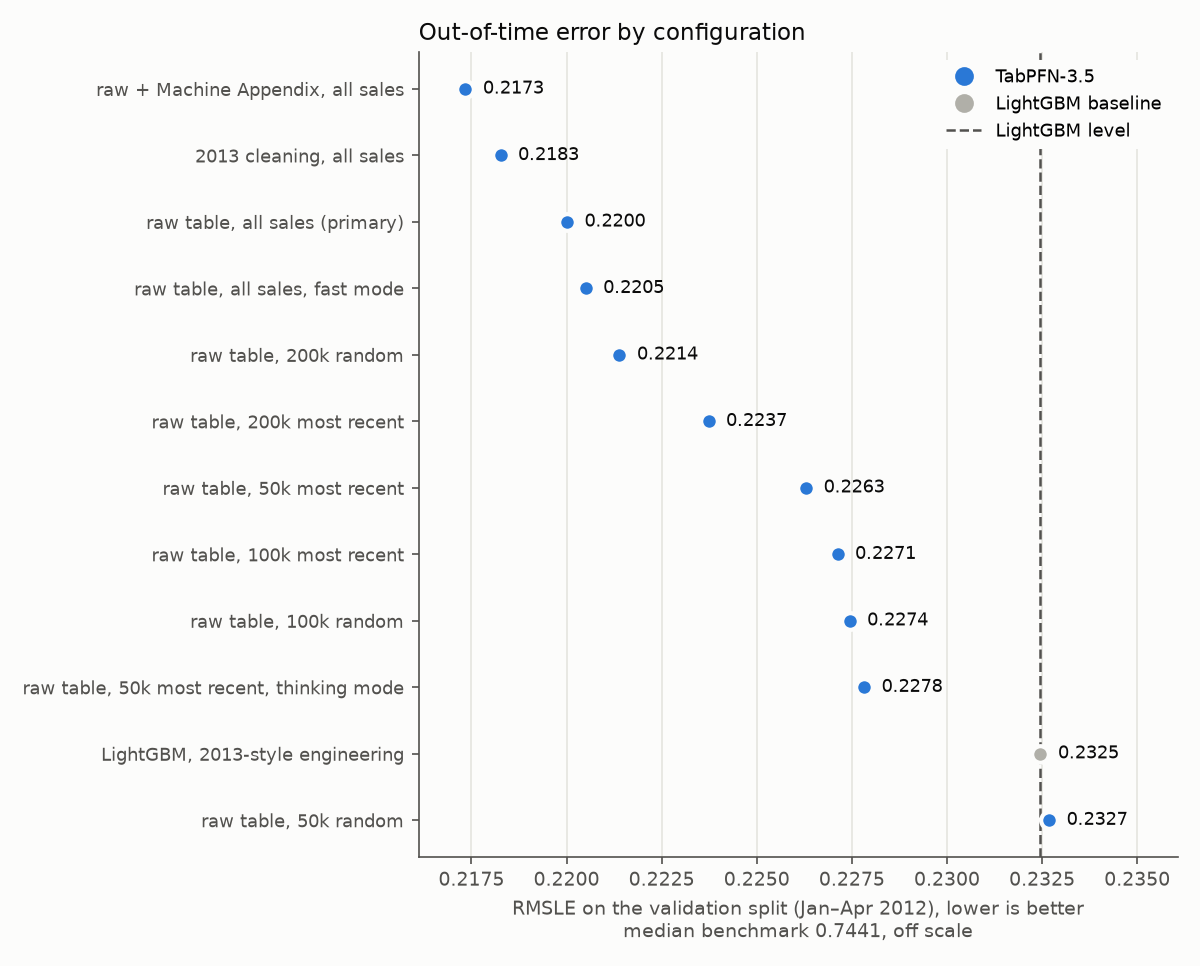
\includegraphics[width=0.82\textwidth]{rmsle_by_run.png}
\caption{Out-of-time RMSLE of each distinct configuration. The dashed line is the engineered LightGBM; the median benchmark (0.7441) is off scale.}
\label{fig:runs}
\end{figure}

\textbf{H1.} The pre-registered claim was the weak one, ``not worse''. The raw table is better, with the whole interval below zero: RMSLE 0.22001 against 0.23246. In a point comparison outside the pre-registration, ten of the eleven distinct TabPFN-3.5 configurations score below the baseline; the exception is a random sample of 50k sales (0.23268).

\textbf{H2.} The clean arm scores 0.21826 and the appendix arm 0.21734, the best configuration overall. Both improvements are real (intervals above zero) but below the 0.005 margin, so H2 survives by the frozen rule; read without the margin, ``cleaning does not improve'' would be false. The gains are about a seventh (cleaning) and a fifth (appendix) of the advantage the raw table already holds over the baseline. The 2013 finding that the appendix did not help \cite{seroussi2014,olariu2013,dataiku2013} is not reproduced in its strong form: with TabPFN-3.5 it helps a little.

\subsection{Context size and recency (H3)}

H3 was stated as a universal claim over context sizes, and the 200k comparison refutes it with an interval entirely above zero (Figure~\ref{fig:context}). With 50k sales the most recent ones clearly win; at 100k the two samplings tie; at 200k a random sample across 23 years of auctions beats the most recent 200k. The two curves meet at all 401,125 sales, the best point by point estimate. For an appraiser the pattern reads like the trade-off in choosing comparables: with few, recency carries the current market; with many, coverage of models and configurations matters more. That reading was not itself tested.

\begin{figure}[H]
\centering
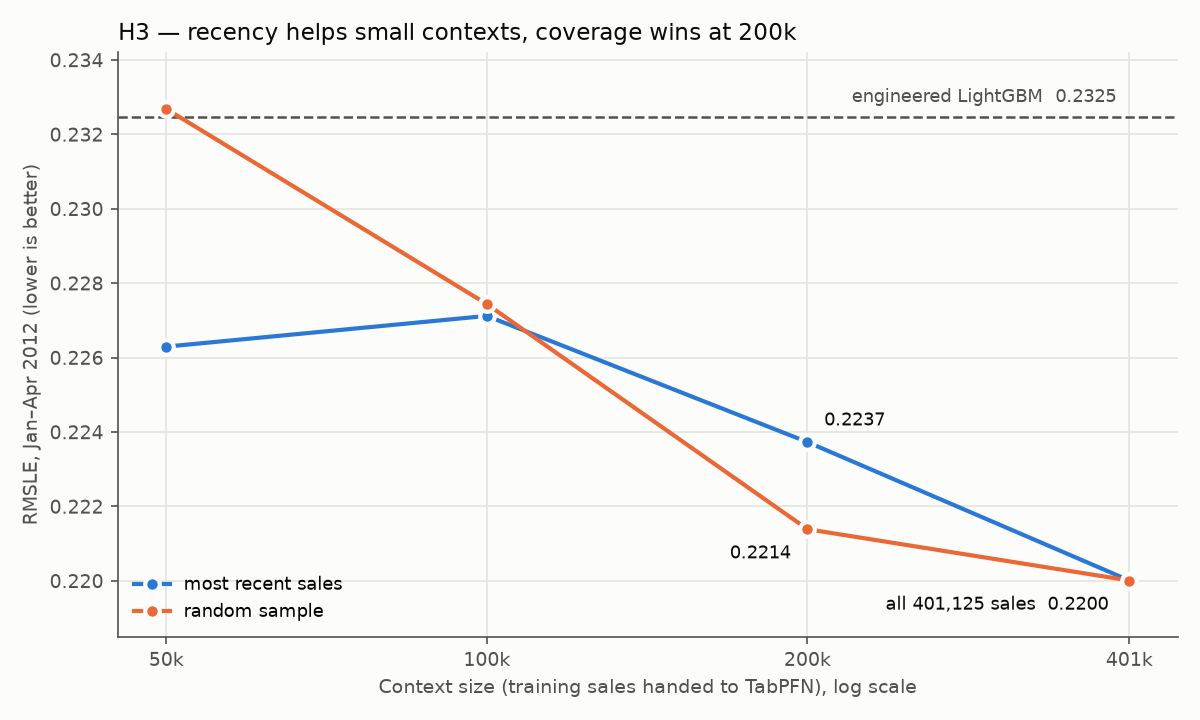
\includegraphics[width=0.78\textwidth]{context_h3.png}
\caption{RMSLE by context size for the most recent sales and for a random sample of equal size.}
\label{fig:context}
\end{figure}

\subsection{Predictive interval (H4)}

The 80\% interval covers 82.0\% of the realized prices four months ahead. All five quantiles sit slightly below the diagonal (Figure~\ref{fig:calib}): 7\%, 19\%, 44\%, 71\% and 89\% of realized prices fall at or below q10, q25, q50, q75 and q90. Realized prices ran 2.6\% above the predictions in geometric mean (mean log residual $+0.0256$). The cause was not tested. A general price rise is not supported, since the January--April median sale price was US\$27,000 in both 2011 and 2012; seasonality is compatible, since in 2009, 2010 and 2011 the January--April median exceeded the full-year median (23,000 vs 22,000; 24,000 vs 23,500; 27,000 vs 26,000).

\begin{figure}[H]
\centering
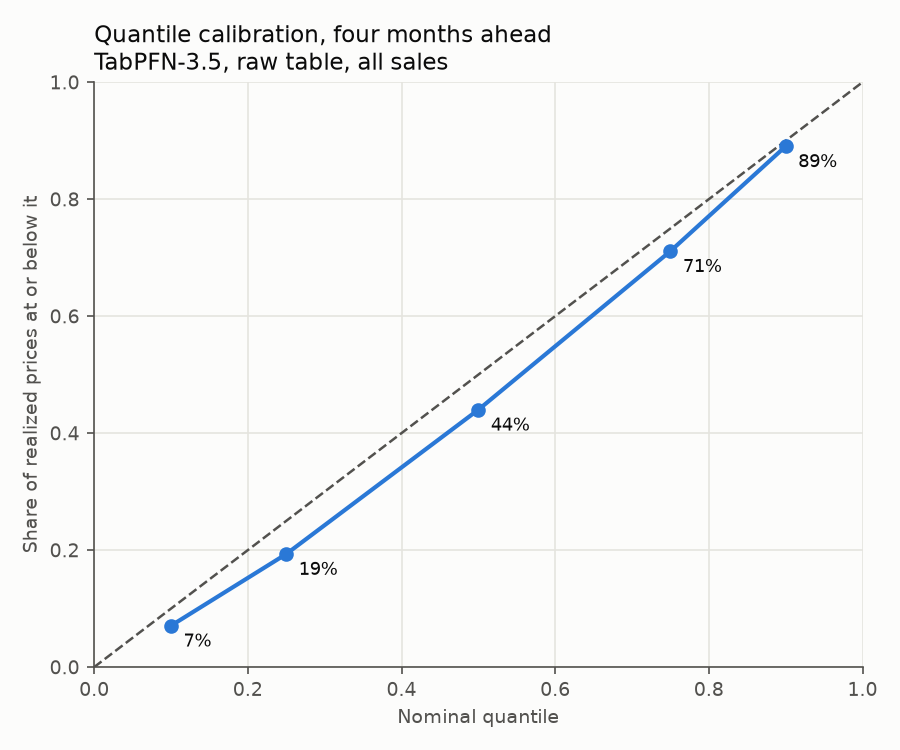
\includegraphics[width=0.55\textwidth]{calibration.png}
\caption{Quantile calibration of the primary run: share of realized prices at or below each predicted quantile.}
\label{fig:calib}
\end{figure}

\subsection{Leaderboard and an external reference (H5)}

The primary RMSLE of 0.22001 is below the 2013 top-10\% mark (0.25339) and numerically below the winning score (0.22909). Those scores were computed by Kaggle on the hidden May--November 2012 test set, by models trained with data through April 2012. Kaggle no longer accepts late submissions, so the comparison is indicative, as pre-registered, and no rank is claimed. The public leaderboard was computed on the same January--April 2012 sales as here, but it is unusable: after the validation prices were released, 108 of 475 teams show an RMSLE of 0.0 on it \cite{parr}.

Parr and Howard \cite{parr} report the only model we found on the same basis: Kaggle's validation set as test set, training on sales through 2011 (from 2007 on). Their tuned random forest, with feature selection and an inflation adjustment, scores 0.2396 (Table~\ref{tab:external}). Their predictions are not available, so the comparison is by point estimate only.

\begin{table}[H]
\centering\small
\caption{Models evaluated on the January--April 2012 sales and trained on sales through 2011.}
\label{tab:external}
\begin{tabular}{lr}
\toprule
Model & RMSLE \\
\midrule
TabPFN-3.5, raw table + Machine Appendix, all sales & 0.21734 \\
\textbf{TabPFN-3.5, raw table, all sales (primary)} & \textbf{0.22001} \\
LightGBM, 2013-style cleaning and features (this study) & 0.23246 \\
Random forest, Parr and Howard \cite{parr} & 0.2396 \\
Median benchmark & 0.74414 \\
\bottomrule
\end{tabular}
\end{table}

\subsection{Exploratory results (not pre-registered)}

\textbf{Fast mode.} With all sales, \texttt{v3.5-fast} scores 0.22050, a difference of $+0.00049$ (95\% CI $[-0.00065, +0.00163]$) against the base model, in 813 s of wall time instead of 1,654 s.

\textbf{Thinking mode.} It failed on the server twice at the planned 200k context and ran at 50k, scoring 0.22782 against 0.22630 for the base model on the same context (difference $+0.00152$, CI $[+0.00033, +0.00274]$). Without a time column, which the API requires as datetimes or numbers while the raw arm keeps the date as text, its internal validation does not use contiguous blocks of time; whether that explains the result was not tested.

\textbf{Reproducibility.} The same 50k configuration, run on two different days, returned identical means and quantiles for all 11,573 sales.

\textbf{Cost.} Usage was read from the API's counter after each block on 2026-10-01. The server quote matched the measured spend exactly for the arms (732,938 tokens, assuming the monthly counter started at zero on October 1) and context (326,828 tokens) blocks; the Kaggle submission block cost twice its quote (730,546 against 365,272), consistent with an automatic client retry but not confirmed. The blocks of that day used 2,357,700 tokens, within a daily limit of 5,000,000.

\section{Discussion}

For valuation practice the main result is that the cleaning step stopped being a prerequisite on this table. A zero-shot model given the auction records as they were published priced the next four months better than a gradient-boosting model given 2013-style cleaning and features, and it delivered predictive intervals that held their nominal coverage. Cleaning and corrected attributes still helped, but by a small amount relative to the advantage already obtained without them. This matters where the data come from many sellers and are never cleaned to a common standard, which is the usual case for equipment auction records.

The refuted hypothesis is as informative as the corroborated ones. A practitioner's instinct, to prefer recent sales, held only when the context was small; with large contexts, breadth won. The small upward bias of the realized prices, with an interval that still held, is a reminder that a model conditioned on past sales can lag the season or market it predicts; here its cause was not established.

Limits are clear. There is one evaluation period, January to April 2012. The baseline is plain: fixed hyper-parameters, no Machine Appendix, no per-group models and no blending, which the 2013 top teams used in whole or in part, so a stronger adversary is possible. There is one table and one market. The hidden test set could not be scored. Deviations from the pre-registration are listed in Appendix~\ref{app:dev}.

\section{Conclusion}

Given the \emph{Blue Book for Bulldozers} table as it was published, TabPFN-3.5 used zero-shot predicted the next four months' auction prices with RMSLE 0.2200, against 0.2325 for a LightGBM with 2013-style cleaning and features and 0.2396 for a published tuned random forest on the same evaluation sales. Four of five pre-registered hypotheses survived; the claim that recent sales are always the better context was refuted at 200,000 sales. Code, results, the pre-registration and the full history of the runs are public.

\section*{Data and code availability}

Code, pre-registration, predictions, metrics, verdicts and figures: \url{https://github.com/abenvenho/tabpfn-bluebook-bulldozers} (Apache-2.0). Data: Kaggle \emph{Blue Book for Bulldozers}, \url{https://www.kaggle.com/c/bluebook-for-bulldozers}, not redistributed. A synthetic smoke test runs the full pipeline with no API access.

\begin{thebibliography}{99}\small\sloppy
\bibitem{breiman2001} L.~Breiman. Random forests. \emph{Machine Learning}, 45(1):5--32, 2001.
\bibitem{dataiku2013} Dataiku. Kaggle contest: Blue Book for Bulldozers. Blog post, 26 April 2013. \url{https://blog.dataiku.com/2013/04/26/kaggle-contest-blue-book-for-bulldozers}.
\bibitem{efron1993} B.~Efron and R.~J. Tibshirani. \emph{An Introduction to the Bootstrap}. Chapman \& Hall, New York, 1993.
\bibitem{friedman2001} J.~H. Friedman. Greedy function approximation: a gradient boosting machine. \emph{The Annals of Statistics}, 29(5):1189--1232, 2001.
\bibitem{hollmann2023} N.~Hollmann, S.~M\"uller, K.~Eggensperger, and F.~Hutter. TabPFN: A transformer that solves small tabular classification problems in a second. In \emph{International Conference on Learning Representations (ICLR)}, 2023.
\bibitem{hollmann2025} N.~Hollmann, S.~M\"uller, L.~Purucker, A.~Krishnakumar, M.~K\"orfer, S.~B. Hoo, R.~T. Schirrmeister, and F.~Hutter. Accurate predictions on small data with a tabular foundation model. \emph{Nature}, 637:319--326, 2025. doi:10.1038/s41586-024-08328-6.
\bibitem{kaggle2013} Kaggle and Fast Iron. Blue Book for Bulldozers. Competition, 2013. \url{https://www.kaggle.com/c/bluebook-for-bulldozers}.
\bibitem{ke2017} G.~Ke, Q.~Meng, T.~Finley, T.~Wang, W.~Chen, W.~Ma, Q.~Ye, and T.-Y. Liu. LightGBM: A highly efficient gradient boosting decision tree. In \emph{Advances in Neural Information Processing Systems 30}, pages 3146--3154, 2017.
\bibitem{olariu2013} A.~Olariu. Trees, ridges and bulldozers made in 1000 AD. Blog post, 2013. \url{http://webmining.olariu.org/trees-ridges-and-bulldozers-made-in-1000-ad/}.
\bibitem{parr} T.~Parr and J.~Howard. \emph{The Mechanics of Machine Learning}, chapter ``Bulldozer testing''. Online book. \url{https://mlbook.explained.ai/bulldozer-testing.html}.
\bibitem{popper1959} K.~R. Popper. \emph{The Logic of Scientific Discovery}. Hutchinson, London, 1959.
\bibitem{priorlabs} Prior Labs. TabPFN (software) and TabPFN-3.5 model card. \url{https://github.com/PriorLabs/TabPFN}; \url{https://huggingface.co/Prior-Labs/tabpfn_3_5}.
\bibitem{seroussi2014} Y.~Seroussi. Fitting noise: forecasting the sale price of bulldozers (Kaggle competition summary). Blog post, 19 November 2014. \url{https://yanirseroussi.com/2014/11/19/fitting-noise-forecasting-the-sale-price-of-bulldozers-kaggle-competition-summary/}.
\end{thebibliography}

\appendix

\section{Deviations from the pre-registration}
\label{app:dev}

\begin{enumerate}
\item \textbf{H5 referee.} Kaggle late submissions turned out to be closed; H5 was rewritten before any run to the leaderboard-mirror comparison.
\item \textbf{Pilot before the context freeze.} A 50k pilot ran before the primary context was frozen. The selection rule was mechanical and already committed, so the pilot could not influence it.
\item \textbf{Primary context.} The rule selected all sales, from the server quote recorded in commit \texttt{442fd3f} before the primary run; a later re-quote gave the same values.
\item \textbf{Modes.} Thinking was moved from the primary context to 200k before any modes run, because of the API cap; it then failed twice server-side and ran at 50k. The fast and thinking model identifiers in the runner were corrected after the H2 arms had run; the base-model path used by every hypothesis was not changed.
\item \textbf{H3 at 100k.} The rule uses the point estimate ($-0.00032$), which counts as supporting, although the interval spans zero. H3 is refuted by the 200k comparison either way.
\item \textbf{H3 rule wording.} The pre-registration writes the rule as ``random $\geq$ recent (diff $\leq 0$)'' without defining \emph{diff}. It was read as in the hypothesis table and the verdict script, both committed before any run. H3 is refuted under either reading.
\item \textbf{Unexplained quota use on 2026-09-30.} The daily quota ran out after the pilot and primary runs, whose quotes add up to about 0.4M tokens; usage was not yet being read, so the rest cannot be attributed.
\end{enumerate}

\section{Settings}

\begin{table}[H]
\centering\small
\begin{tabular}{p{5.2cm}p{9.6cm}}
\toprule
Item & Value \\
\midrule
TabPFN client & \texttt{tabpfn-client} 0.6.1, default settings, server default model (v3.5) \\
Quantiles & 0.10, 0.25, 0.50, 0.75, 0.90 \\
Cost quote per call (pricing \texttt{quota\_v3}) & all sales 181,897; 200k 53,211; 100k 18,496; 50k 10,000 tokens \\
LightGBM & 4.7.0; learning rate 0.05; 128 leaves; min. 20 per leaf; 0.8 column/row sampling \\
LightGBM trees & early stopping, patience 200, max. 5,000; selected 995; 55 features \\
Bootstrap & 10,000 paired resamples, seed 42, percentile 95\% interval \\
Environment & Python 3.11+, versions pinned in \texttt{requirements.txt} \\
\bottomrule
\end{tabular}
\end{table}

\end{document}
